\documentclass[
    %uninadraft,
    %colorlinks, 
    blacklinks,
    %palatino,
    libertine,
    %mathpazo,
    %tgschola,
    %tgscholamathpazo,
    %alegreya
]{uninathesis}

%\AtBeginDocument{\addtocontents{toc}{\protect\thispagestyle{empty}}} %remove page number from toc

\usepackage[english]{babel}
\addto\captionsenglish{% Replace "english" with the language you use
  \renewcommand{\contentsname}%
    {\sffamily Contents}%
}

% Math
\RequirePackage{mathtools}
\RequirePackage{mathrsfs} %need this for mathscr
\let\openbox\relax
\RequirePackage{amsthm}
\RequirePackage{stmaryrd} %for \llbracket

\theoremstyle{plain}
\newtheorem{theorem}{Theorem}

\theoremstyle{definition}
\newtheorem{definition}{Definition}
\newtheorem{example}{Example}

% Tikz - may be removed if unneeded
\RequirePackage{tikz}
\RequirePackage{pgfplots}
\pgfplotsset{compat=1.16}
\usetikzlibrary{positioning,automata,calc,fit,shapes,backgrounds,arrows.meta}
\usepackage{makecell}

% Miscellanea Packages
\RequirePackage[utf8]{inputenc}
\usepackage{ marvosym } %/Lightning
%\usepackage{ stmaryrd } %/lightning
%\usepackage[htt]{hyphenat}
\usepackage{subcaption} %subfigures

% read configuration file
%double quote command
\newcommand\dquote[1]{``#1''}
\newcommand\dquoteit[1]{``\emph{#1}''}

%single quote command
\newcommand\squote[1]{`#1'} %can write your macros here

% Bibliography
\RequirePackage{csquotes}
\RequirePackage[sorting=none,maxbibnames=4]{biblatex} %dashed=false to remove dashes on repeated authors.
\bibliography{_bib/bibliography.bib} %bib database(s)

% Front page (package uninafrontespizio)
\Universita{Università degli Studi di Napoli Federico II}
\Facolta{Scuola Politecnica e delle Scienze di Base}
\Dipartimento{Dipartimento di Ingegneria Elettrica e Tecnologie dell'Informazione}
\CorsoDiLaurea{Corso di Laurea Magistrale in Informatica}
%\Materia{Verifica di Sistemi}
\AnnoAccademico{2024--2025}
\Titolo{Implementation of a decision procedure for the fluted fragment in Vampire}
\Relatore{Prof.\ Fabio \textsc{Mogavero}}
\Relatore{Prof.\ Massimo \textsc{Benerecetti}}
% \Relatore{Baronessa Filiguelli \textsc{de Bonchamps}}
\RelatoreLabel{Relatori}
\CorrelatoreLabel{}
\Candidato{Riccardo \textsc{Elena}}
\Matricola{N86/4490}
\Logo{logo-federico-II.pdf}
\LogoWidth{3.5cm}
\LogoPosition{below-uni}

%custom hyphenation
\hyphenation{ERTMS/ETCS}

\usepackage[title,titletoc]{appendix}

\begin{document}

    \pagestyle{empty}
    \frontmatter
    \makefrontespizio~\clearpage
    \makefrontespizioalt~\clearpage

    \pagestyle{backmatter}
    \chapter*{Abstract}

% This is the abstract.\blindtext[2]

% \chapter*{Sommario}
% Qui puoi inserire il sommario (la traduzione dell'abstract in italiano).
% \blindtext[2]
    
    \clearpage
    \tableofcontents

    \mainmatter{}

    \newpage\pagestyle{introduction}

% The \unnumberedchapter, \unnumberedsection commands provided by the uninathesis 
% documentclass add an unnumbered entry to the TOC.
% If you use the starred version of classic sectioning commands (e.g. \chapter*)
% no TOC entry will be added!

\chapter*{Introduction}
% \unnumberedsection{A first unnumbered section}

First-Order Logic (FOL) emerged from the mathematical foundations laid in \textit{Begriffsschrift}~\cite{frege1879} by \citeauthor{frege1879} and in \textit{Principia Mathematica}~\cite{russell1910} by \citeauthor{russell1910}, and has since become a cornerstone formalism in computer science.
Its formal yet expressive nature makes it particularly well-suited for computational reasoning across diverse domains.
In knowledge representation, FOL underpins semantic web technologies and ontology languages like OWL, enabling machines to reason about complex relationships in data.
Meanwhile, in verification, it serves as the logical foundation for model checkers and theorem provers that ensure software correctness, while in artificial intelligence, it historically powered automated reasoning systems and planning algorithms, though modern AI has largely shifted toward statistical and neural approaches that often lack the transparency and formal guarantees that FOL-based systems provide.

However, the expressive power of FOL comes at a cost: undecidability.
This was established independently in the 1930s by \citeauthor{church1936}~\cite{church1936} using the lambda calculus, and by \citeauthor{turing1936}~\cite{turing1936} via Turing machines---two distinct formalisms that captured the limits of computation.
Their results demonstrated that no algorithm can, in general, determine whether an arbitrary FOL formula is valid. This fundamental limitation creates a significant computational barrier for automated reasoning.
In response, two complementary research directions have emerged: the systematic identification of decidable fragments that retain sufficient expressiveness for practical applications, and the development of automated theorem provers (ATPs) that---while unable to guarantee termination on all inputs---employ sophisticated heuristics and optimizations to solve many real-world problems efficiently.

Among the most prominent ATPs for first-order logic is \textit{Vampire}~\cite{kovacs2013vampire}, a high-performance prover built on advanced saturation-based reasoning.
Vampire combines ordered resolution with literal selection, term indexing, and clause simplification techniques to explore the space of logical consequences efficiently.
It also incorporates modern enhancements such as efficient preprocessing, strategy scheduling, and support for first-order logic with built-in theories.
These features have made Vampire highly successful in competitive settings like the CADE ATP System Competition (CASC)\footnote{The CADE ATP System Competition (CASC) is the annual evaluation of fully automatic, classical logic, ATP systems --- the world championship for such systems.}, and effective in practical applications ranging from formal verification to software analysis.
Moreover, Vampire's extensible architecture and open-source nature make it the go-to choice for research and experimentation in the field of automated reasoning.

While general-purpose provers like \textit{Vampire} are designed to handle unrestricted first-order logic, certain decidable fragments offer opportunities for more targeted and efficient reasoning.
One such fragment is the \emph{Fluted Fragment}, distinguished by its strict syntactic discipline: variables in atomic formulas must follow the order in which they are quantified~\cite{quine1968predicate}.
This constraint, first introduced by Quine, limits expressiveness in some dimensions but crucially preserves decidability. Subsequent studies have shown that the Fluted Fragment occupies an interesting middle ground—more complex than many guarded or bounded-variable fragments, yet still admitting well-characterized decision procedures~\cite{pratt2019fluted}.
Applications have emerged in areas such as knowledge representation, database logic and computational linguistics, where the fragment’s regular structure aligns naturally with hierarchical or sequential data.
\uninatodo{I remember we discussed this application, but I cannot find the reference now.}
These properties make it a compelling candidate for specialized reasoning techniques that can outperform general ATPs in relevant domains.

A specialized reasoning technique for the Fluted Fragment is presented by \citeauthor{schmidt2000resolution} in their resolution-based decision procedure~\cite{schmidt2000resolution}.
Their approach characterizes fluted logic through a novel class of \emph{fluted clauses}, and introduces a calculus ---\textsc{R\textsuperscript{sep}}--- which extends ordered resolution with a dynamic renaming rule called \emph{separation}.
This rule enables the transformation of non-strongly fluted clauses into strongly fluted ones, thereby preserving a bounded number of variables and ensuring closure under resolution.
Crucially, the authors prove that their calculus is sound, complete, and terminating for fluted logic, establishing a resolution-based decision procedure for the fragment.

%This result not only deepens the understanding of the structural properties that make fluted logic decidable, but also provides a foundation for building dedicated automated reasoning tools that leverage the syntactic discipline of the fragment.

In this thesis, we implement this resolution-based decision procedure for the Fluted Fragment, with the goal of evaluating its practical effectiveness.
By faithfully realizing the \textsc{R\textsuperscript{sep}} calculus, including the separation rule and associated structural constraints, the implementation provides a concrete instantiation of the theoretical framework.
To assess the impact of fragment-specific optimization, we conduct an empirical comparison against the general-purpose theorem prover \textit{Vampire}, highlighting the potential advantages of tailored reasoning techniques for decidable fragments of first-order logic.

\unnumberedsection{About this thesis work}

This thesis retraces all the steps of the implementation of the resolution-based decision procedure for the Fluted Fragment mentioned above, starting from the theoretical foundations and culminating in the empirical evaluation of the implemented system.

The work is structured as follows:

\begin{description}
    \item[Chapter 1] provides an overview of the theoretical foundations of first-order logic, briefly discussing its structure and key concepts such as Skolemization, Naming, and Clausification.
    \item[Chapter 2] illustrates the main inference rules of a resolution-based decision procedure, highlighting the differences between their standard and their ordered versions. In particular, it covers the concept of \textit{liftable orders} and how they can be used for the definition of \textit{ordered inference rules}.
    \item[Chapter 3] describes the Fluted Fragment and the resolution-based decision procedure for it, detailing the separation rule and the structural constraints that ensure decidability. The chapter discusses the structure of the fluted formulae, the definition of fluted clauses, and the naming procedure that ensures the flutedness of the clauses.
    \item[Chapter 4] briefly analyses \textit{Vampire} and its architecture, focusing on relevant components for the implementation of the decision procedure. In detail, it discusses the \textit{Preprocessor}, the \textit{Saturation Algorithm}, and the \textit{Clause Selection} components.
    \item[Chapter 5] presents the implementation of the decision procedure, discussing the design choices made, and the challenges encountered during development, divided into three main parts covering the three main components of the implementation: the \textit{Classifier}, the \textit{Preprocessor}, and the \textit{Fluted Resolution}.
    \item[Chapter 6] discusses the results of the first evaluation, based on the TPTP library, highlighting the strengths and weaknesses of the implemented decision procedure. These problems have been selected using the \textit{Classifier} component and the evaluation is based on the comparison with the results of \textit{Vampire} and of a \textit{Hybrid model}, composed by the \textit{Fluted Preprocessor} and the \textit{Vampire Resolution}, on the same problems.
    \item[Chapter 7] discusses the results of the second evaluation, based on the automatically generated problems, as well as the design and implementation process of the problems generator and the evaluation framework. This evaluation required the implementation of another component, the \textit{Fluted Generator}, which is responsible for generating the problems to be solved by the decision procedure and by the other \textit{two models}.
    \item[Chapter 8] concludes the thesis, summarizing the main findings and discussing potential future work.
\end{description}





    \newpage\pagestyle{main}

    \chapter{First Order Logic}\label{chap:first}

\inlineminitoc{}

\noindent First-order logic (FOL), or predicate logic, is a formal system used in mathematics, philosophy, linguistics, and computer science to express statements about objects and their relationships.
It uses \textbf{terms} for the representation of objects in the domain of discourse and \textbf{predicates} to express properties of these objects or relationships between them.
Moreover, FOL allows for the use of \textbf{quantifiers} to make statements that apply to all objects (universal quantification) or some objects (existential quantification) in the domain, and \textbf{logical connectives} to construct more complex statements.

One well-known informal statement, \dquote{All humans are mortal} for example, can be expressed in FOL as:
\begin{equation*}
    \forall x \left( \text{H}(x) \implies \text{M}(x) \right)
\end{equation*}

Syntactically speaking, this sentence is composed of:
\begin{itemize}
    \item a \textbf{quantifier} \(\forall\)
    \item a \textbf{variable} \(x\) which ranges over the whole domain of discourse (possibly every object in the universe)
    \item a \textbf{unary predicate} \(\text{H}\) applied to \(x\)
    \item a \textbf{unary predicate} \(\text{M}\) applied to \(x\)
    \item a \textbf{logical connective} \(\implies\)
\end{itemize}

Upon this syntactic structure, we can build a semantic interpretation, which assigns meaning to the symbols used in the sentence.
In this case, we can interpret \(\text{H}(x)\) as \dquote{\(x\) is a human} and \(\text{M}(x)\) as \dquote{\(x\) is mortal}.
Moreover, the universal quantifier \(\forall\) indicates that the statement applies to all objects in the domain of discourse.
The connective \(\implies\) is the \textit{material implication} of \textit{propositional logic}, indicating that if the first part is true, then the second part must also be true.

As we can see, using FOL we can divide the statement into its syntactic and semantic components, which allows us to reason about its structure separately from its meaning.
This separation permits us to generalize the reasoning process to other statements with similar structures and to deduce new statements solely from the syntactic structure.
This makes FOL particularly suitable for computational treatment: automated systems can manipulate the syntactic form of statements while guaranteeing that these manipulations reflect valid semantic consequences in all interpretations — a property known as \textit{soundness}, \citeauthor{enderton2001}~\cite{enderton2001}.

As we will see later, this clear separation is crucial for the development of automated reasoning systems, such as the Vampire theorem prover, because it allows us to convert the reasoning task into a syntactic manipulation task, treating statements as symbolic strings with a specific syntax, without the need to explicitly encode the meaning of each statement.

In order to preserve the truth value of statements during this manipulation process, we cannot rely on the syntactic structure alone; we must define a set of rules that act only on the syntactic structure while ensuring truth preservation.
This set of rules is called \textbf{inference rules}, and they allow us to derive new statements from existing ones without altering their truth value.
\section{From Terms to Sentences}

First and foremost, we need to rigorously define the structure of first-order logic.
The most basic building blocks of FOL are \textbf{terms}, which represent objects in the domain of discourse.
Those are variables (\(x,y,z\)), functions (\(f,g,h\)) and  symbols (\(a,b,c\)), sometimes viewed as function symbols with arity 0.
Variables are placeholders that can represent any object in the domain, while constants refer to specific objects. Functions map objects to other objects, allowing for more complex expressions.

Terms alone do not constitute statements in FOL, as they lack an associated \textit{truth value}.
The main focus of FOL is on \textbf{predicates} (\(P,Q,R\)) ---so the name \textit{predicate logic}---, which are used to express properties of objects or relationships between them.
Examples of predicates include \(\text{H}(x)\) for \dquote{is a human} or \(\text{M}(x)\) for \dquote{is mortal}.


Predicates are applied to terms to form \textbf{atomic formulae} (\(A,B\)), the basic units of meaning in FOL\@. They serve as the building blocks of more complex and structured statements, called \textbf{formulae} \(\phi, \psi\), obtained by combining atomic formulae using logical connectives and quantifiers.

Solely, not even atomic formulae always bear a truth value, as they can contain \textit{free variables}, namely variables that are not bound by a quantifier. These variables do not refer to any specific object in the domain, and thus the truth value of the atomic formula depends on the interpretation of these variables.
This ambiguity can be illustrated with natural language; for instance, the statement \dquote{X is a human} does not clearly state \textit{which} object \(X\) has to be a human to make the statement true.
The quantifiers resolve this ambiguity by specifying the scope of the variable \(X\). Indeed, the statement \dquote{For all X, X is a human} clearly has a truth value, as it asserts something about every object, whether it is true or not.
Only (atomic) formulae with all variables bound can be said to have a definite truth value, and those are called (\textbf{atomic}) \textbf{sentences}.

Last but not least, to combine (atomic) formulae/sentences into more complex expressions, we can use logical connectives. Those are symbols that applied to one or more formulae yield a new formula, whose truth value depends on the truth values of the original formulae and on the semantics of the connective.
In particular, the principal connectives used in FOL are:

\begin{itemize}
  \item \textbf{Negation} (\(\neg\)): This connective takes a single formula and \textbf{inverts} its truth value.
  \item \textbf{Conjunction} (\(\land\)): This connective combines two formulae and is \textbf{true} if both are true.
  \item \textbf{Disjunction} (\(\lor\)): This connective combines two formulae and is \textbf{true} if at least one is true.
  \item \textbf{Implication} (\(\implies\)): This connective expresses a conditional relationship between two formulae. The new formula is \textbf{false} only if the first formula is true and the second formula is false.
  \item \textbf{Biconditional} (\(\iff\)): This connective expresses an equivalence between two formulae. The new formula is \textbf{true} if both formulae have the same truth value.
\end{itemize}

A \textbf{literal} is either a positive atomic formula or a negated atomic formula.

\subsection{Syntax}

The syntax of FOL formulae can be formalized with a \textit{context free grammar} (CFG).
In particular, being \(\mathcal{V}\) the set of all variables, \(\mathcal{C}\) the set of all constants, \(\mathcal{F}\) the set of all function symbols, \(\mathcal{P}\) the set of all predicate symbols, we can define the grammar as follows:

\begin{equation}
  FOL = \left( V , \Sigma, \phi \in V, R\right)
\end{equation}
where:
\begin{itemize}
  \item \(V = \{\tau, \alpha, \phi\}\)
  \item \(\Sigma = \mathcal{V} \cup \mathcal{C} \cup \mathcal{F} \cup \mathcal{P} \cup \{\forall, \exists, \land, \lor, \neg, \implies, \iff, \left(,\right), \top, \bot\}\)
   \item \(R\) = \begin{flalign}
    \begin{aligned}
      \tau \rightarrow \ms &x \in \mathcal{V} \ms|\ms 
                        c \in \mathcal{C} \ms|\ms 
                        f(\tau,\ldots,\tau) \in \mathcal{F} \\
      \alpha \rightarrow \ms &P(\tau,\ldots,\tau), P \in \mathcal{P} \\
      \phi \rightarrow \ms & \ms|\ms \alpha \ms|\ms \top \ms|\ms \bot \ms|\ms 
       \neg\phi \ms|
       \left(\phi\land\phi\right) |
       \left(\phi\lor\phi\right) |
       \left(\phi\implies\phi\right) |
       \left(\phi\iff\phi\right) | \ms
       \forall x\left(\phi\right) \ms|\ms
       \exists x\left(\phi\right)
    \end{aligned} &&
  \end{flalign}
\end{itemize}

The language generated by this grammar is the set of all \textit{well-formed formulae} in FOL\@.

Every string of the so generated language can also be represented with a \textit{syntactic tree}, which is a tree representation of the syntactic structure of the formula, highlighting the hierarchical relationships between its components.

An example of a syntactic tree for the formula \(\forall x \left(\text{H}(x) \implies \text{M}(x)\right)\) is shown in Figure~\ref{fig:syntactic_tree}.

\begin{figure}[H]
    \centering
    \begin{tikzpicture}[syntree]
        \node[quantifier] {{\(\forall x\)}}
            child { node[connective] {\(\implies\)} 
              child { node[literal] {\(\text{H}(x)\)} }
              child { node[literal] {\(\text{M}(x)\)} }
            };
    \end{tikzpicture}
    \caption{Syntactic tree for \(\forall x (\text{H}(x) \implies \text{M}(x))\)}\label{fig:syntactic_tree}
\end{figure}

In this representation, it is possible to omit the parentheses around the subformulae, as the tree structure already encodes the necessary grouping.

Moreover, is possible to isolate a \textit{subgrammar} by considering only the rules that generate atomic formulae (excluding so the ones deriving from \(\phi\)). Doing this easily allows to define the concept of \textbf{subterm} as a \textit{proper subtree} of the syntactic tree that represents an atomic formula (or by extension a literal).

An example of such a tree is shown in Figure~\ref{fig:subterm_tree} for the atomic formula \(P(f(x, g(y)))\).
\begin{figure}[H]
    \centering
    \begin{tikzpicture}[syntree]
        \node[literal] {\(P\)}
            child { node[literal] {\(f\)}
              child { node[literal] {\(x\)} }
              child { node[literal] {\(g\)}
                child { node[literal] {\(y\)} }
              }
            };
    \end{tikzpicture}
    \caption{Syntactic tree for the atomic formula \(P(f(x, g(y)))\) showing nested function structure}\label{fig:subterm_tree}
\end{figure}

If we consider multiple atomic formulae (or literals), is possible to represent them as a \textbf{forest} of syntactic trees, where each tree represents an atomic formula.

\begin{figure}[H]
    \centering
    \begin{minipage}[t]{0.48\textwidth}
        \centering
        \begin{tikzpicture}[syntree]
            \node[literal] {\(P\)}
                child { node[literal] {\(f\)}
                  child { node[literal] {\(x\)} }
                  child { node[literal] {\(g\)}
                    child { node[literal] {\(y\)} }
                  }
                };
        \end{tikzpicture}
    \end{minipage}
    \hfill
    \begin{minipage}[t]{0.48\textwidth}
        \centering
        \begin{tikzpicture}[syntree]
            \node[literal] {\(\neg P\)}
                  child { node[literal] {\(f\)}
                    child { node[literal] {\(x\)} }
                    child { node[literal] {\(g\)}
                      child { node[literal] {\(y\)} }
                    }
                  };
        \end{tikzpicture}
    \end{minipage}
    \caption{Forest of the literals \(P(f(x, g(y)))\) and \(\neg P(f(x, g(y)))\)}\label{fig:subterm_forest}
\end{figure}

% Add a line to introduce DAG representation and explain why in practice it's better
In practice, it is often more convenient to represent these structures as Directed Acyclic Graphs (DAGs) rather than trees. This is because DAGs allow for the sharing of subterms, which can lead to more compact representations and easier manipulation of the formulae.

DAGs can be particularly useful in automated reasoning and theorem proving, where the same subterm may appear in multiple places within a formula. By representing the formula as a DAG, we can avoid redundant copies of the subterms and simplify the reasoning process.

\begin{figure}[H]
    \centering
    \begin{tikzpicture}[syntree]
        % Livello delle variabili (condivise)
        \node[literal] (x) at (0,0) {\(x\)};
        \node[literal] (y) at (2,0) {\(y\)};
        
        % Livello delle funzioni (condivise)
        \node[literal] (g) at (2,1) {\(g\)};
        \node[literal] (f) at (1,2) {\(f\)};
        
        % Livello dei predicati (separati)
        \node[literal] (P_pos) at (-0.5,3) {\(P\)};
        \node[literal] (P_neg) at (2.5,3) {\(\neg P\)};
        
        % Connessioni condivise
        \draw[-latex, thick] (g) -- (y);
        \draw[-latex, thick] (f) -- (x);
        \draw[-latex, thick] (f) -- (g);

        % Connessioni per literal positivo
        \draw[-latex, thick] (P_pos) -- (f);

        % Connessioni per literal negativo
        \draw[-latex, thick] (P_neg) -- (f);


        % Etichette
        \node[left=0.3cm of P_pos, font=\footnotesize] {\(P(f(x, g(y)))\)};
        \node[right=0.3cm of P_neg, font=\footnotesize] {\(\neg P(f(x, g(y)))\)};
        
        % Evidenzia i nodi condivisi con colore diverso
        \node[literal] at (x) {\(x\)};
        \node[literal] at (y) {\(y\)};
        \node[literal] at (g) {\(g\)};
        \node[literal] at (f) {\(f\)};
    \end{tikzpicture}
    \caption{DAG representation showing shared subterms between \(P(f(x, g(y)))\) and \(\neg P(f(x, g(y)))\)}\label{fig:subterm_dag}
\end{figure}

\subsection{Semantics}

To formalize semantics in FOL, we need to define the meaning of the symbols and the truth conditions for the formulae. This is typically done using a \textit{model}, which consists of a domain of discourse and an interpretation function that assigns meanings to the constants, functions, and predicates.

A \textbf{model} for a FOL language is a pair \(M = (D, I)\), where:
\begin{itemize}
  \item \(D\) is a non-empty set, called the \textbf{domain of discourse}.
  \item \(I\) is an interpretation function that assigns:
  \begin{itemize}
    \item Each constant \(c \in \mathcal{C}\) to an element \(I(c) \in D\).
    \item Each function symbol \(f \in \mathcal{F}\) to a function \(I(f): D^{n_f} \to D\), where \(n_f\) is the arity of \(f\).
    \item Each predicate symbol \(P \in \mathcal{P}\) to a relation \(I(P) \subseteq D^{n_P}\), where \(n_P\) is the arity of \(P\).
  \end{itemize}
\end{itemize}

The truth value of a formula \(\phi\) in a model \(M\) is determined by the interpretation function and the structure of the formula as follows:

\subsubsection{Variable Assignment}\label{subsubsec:variable_assignment}
Given a model \(M = (D, I)\), a \textbf{variable assignment} (or \textbf{valuation}) is a function \(\sigma: \mathcal{V} \to D\) that assigns each variable to an element of the domain. We denote by \(\sigma[x \mapsto d]\) the assignment that is identical to \(\sigma\) except that it maps variable \(x\) to element \(d \in D\).

\subsubsection{Term Evaluation}
The \textbf{evaluation} of a term \(t\) in model \(M\) under assignment \(\sigma\), denoted \(\llbracket t \rrbracket_M^\sigma\), is defined recursively:
\begin{itemize}
  \item If \(t\) is a variable \(x\), then \(\llbracket x \rrbracket_M^\sigma = \sigma(x)\).
  \item If \(t\) is a constant \(c\), then \(\llbracket c \rrbracket_M^\sigma = I(c)\).
  \item If \(t = f(t_1, \ldots, t_n)\) where \(f\) is an \(n\)-ary function symbol, then 
        \[\llbracket f(t_1, \ldots, t_n) \rrbracket_M^\sigma = I(f)(\llbracket t_1 \rrbracket_M^\sigma, \ldots, \llbracket t_n \rrbracket_M^\sigma)\]
\end{itemize}

\subsubsection{Truth Conditions}
The \textbf{satisfaction} of a formula \(\phi\) in model \(M\) under assignment \(\sigma\), denoted \(M, \sigma \models \phi\), is defined recursively:

\begin{itemize}
  \item \textbf{Atomic formulae:}
  \begin{itemize}
    \item \(M, \sigma \models P(t_1, \ldots, t_n) \leftrightarrow (\llbracket t_1 \rrbracket_M^\sigma, \ldots, \llbracket t_n \rrbracket_M^\sigma) \in I(P)\)
    \item \(M, \sigma \models \top\) (always true)
    \item \(M, \sigma \not\models \bot\) (never true)
  \end{itemize}
  
  \item \textbf{Logical connectives:}
  \begin{itemize}
    \item \(M, \sigma \models \neg \phi \leftrightarrow M, \sigma \not\models \phi\)
    \item \(M, \sigma \models \phi \land \psi \leftrightarrow M, \sigma \models \phi\) and \(M, \sigma \models \psi\)
    \item \(M, \sigma \models \phi \lor \psi \leftrightarrow M, \sigma \models \phi\) or \(M, \sigma \models \psi\)
    \item \(M, \sigma \models \phi \implies \psi \leftrightarrow M, \sigma \not\models \phi\) or \(M, \sigma \models \psi\)
    \item \(M, \sigma \models \phi \iff \psi \leftrightarrow \left(M, \sigma \models \phi \text{ and } M, \sigma \models \psi\right) \text{ or } \left(M, \sigma \not\models \phi \text{ and } M, \sigma \not\models \psi\right)\)
  \end{itemize}
  
  \item \textbf{Quantifiers:}
  \begin{itemize}
    \item \(M, \sigma \models \forall x \ms \phi\) if and only if for all \(d \in D\), \(M, \sigma[x \mapsto d] \models \phi\)
    \item \(M, \sigma \models \exists x \ms \phi\) if and only if there exists some \(d \in D\) such that \(M, \sigma[x \mapsto d] \models \phi\)
  \end{itemize}
\end{itemize}

\subsubsection{Semantic Notions}
A formula \(\phi\) is:
\begin{itemize}
  \item \textbf{Satisfiable} if there exists a model \(M\) and assignment \(\sigma\) such that \(M, \sigma \models \phi\).
  \item \textbf{Valid} (sometimes called a \textbf{tautology}) if for all models \(M\) and assignments \(\sigma\), \(M, \sigma \models \phi\). We write \(\models \phi\).
  \item \textbf{Unsatisfiable} (or \textbf{contradictory}) if for all models \(M\) and assignments \(\sigma\), \(M, \sigma \not\models \phi\).
\end{itemize}

For a set of formulae \(\Gamma\) and a formula \(\phi\), we say \(\Gamma\) \textbf{semantically entails} \(\phi\), written \(\Gamma \models \phi\), if for all models \(M\) and assignments \(\sigma\):
  \[M, \sigma \models \psi \rightarrow M, \sigma \models \phi,\ms \text{for all } \psi \in \Gamma\]


\section{Substitutions and Unification}
In Section~\ref{subsubsec:variable_assignment} we introduced the notation \(\sigma[x \mapsto d]\) to indicate a variable assignment in the semantic evaluation of a formula. We now extend this concept to the purely \emph{syntactic} setting, where variables are replaced by \emph{terms} rather than by elements of the interpretation domain. This leads to the notions of \emph{substitution}, \emph{unification}, and \emph{most general unifier}.

\subsection{Substitutions}
Given a term or literal \(\tau\), the notation \(\tau[x_k \mapsto t]\) denotes the expression obtained by replacing every occurrence of the variable \(x_k\) in \(\tau\) with the term \(t\).  
For example, if \(\tau = g(x_1, x_2)\), then:
\begin{equation}
\tau[x_1 \mapsto h] = g(h, x_2)
\end{equation}

A \textbf{substitution} is a function mapping a subset of variables \(\mathcal{V}^{'} \subseteq \mathcal{V}\) to a set of terms \(\mathcal{T} \subseteq \mathcal{V} \cup \mathcal{F} \cup \mathcal{C}\):
\begin{equation}
\sigma = \{ (x_1, t_1), \ldots, (x_n, t_n) \}
\end{equation}
If \(\tau\) is a term and \(\sigma\) is a substitution, we write \(\tau\sigma\) or \(\tau[x_1 \mapsto t_1, \ldots, x_n \mapsto t_n]\) for the term obtained by replacing all \(x_i\) with \(t_i\) \emph{simultaneously}.  
The word “simultaneously” means that each replacement is made with respect to the \emph{original} \(\tau\), without the effect of one replacement influencing another.

For instance, if \(\tau = f(x_1, x_2)\), then:
\begin{equation}
\tau[x_1 \mapsto x_2, \ms x_2 \mapsto x_1] = f(x_2, x_1)
\end{equation}
and not \(f(x_1, x_1)\), which would arise from sequential application.

\subsection{Generality of  Substitutions}
For two substitutions \(\sigma_1\) and \(\sigma_2\), we say \(\sigma_1\) is \textbf{more general} than \(\sigma_2\) if for every term \(\tau\) there exists a substitution \(\theta\) such that:
\begin{equation}  
  \tau\sigma_2 = (\tau\sigma_1)\theta
\end{equation}

If there is a substitution \(\sigma\) with:
\begin{equation}
\tau_1\sigma = \tau_2\sigma
\end{equation}
then \(\tau_1\) and \(\tau_2\) are said to be \textbf{unifiable}, and \(\sigma\) is called a \textbf{unifier}.

A unifier \(\sigma\) for two terms \(\tau_1\) and \(\tau_2\) is called a \textbf{most general unifier} (MGU) if it is more general than any other unifier of \(\tau_1\) and \(\tau_2\).

\subsection{Unification Beyond Single Terms}
The unification concept extends to sets of terms, literals, and sets of literals.  
A set of terms \(\mathcal{T}\) is \textbf{unifiable} if there exists a substitution \(\sigma\) such that for any \(\tau_i, \tau_j \in \mathcal{T}\) we have \(\tau_i\sigma = \tau_j\sigma\). In this case, \(\sigma\) is a unifier of \(T\).

Two literals with the same arity:
\begin{equation}
L_1 = P(\tau_1, \ldots, \tau_n), \quad L_2 = \neg P(\tau'_1, \ldots, \tau'_n)
\end{equation}
are unifiable if there is a substitution making them identical, disregarding negation. Equivalently, if \(f\) is a fresh \(n\)-ary function symbol, then \(L_1\) and \(L_2\) are unifiable if and only if \(f(\tau_1, \ldots, \tau_n)\) and \(f(\tau'_1, \ldots, \tau'_n)\) are unifiable.  
Literals of different arities are never unifiable.

\subsection{Obstructions to Unification}
When attempting to unify two terms, two main forms of obstruction can occur:
\begin{enumerate}
    \item \textbf{Function obstruction:} in a parallel traversal of the syntactic trees of both terms, two different function symbols occur at corresponding positions. For example:
    \[
    f(x_1, g_1(x_2)) \quad\text{and}\quad f(x_1, g_2(x_2))
    \]
    are not unifiable because \(g_1 \neq g_2\).
    \item \textbf{Variable obstruction:} in a parallel traversal, a variable \(x\) appears in one term while the other term contains a subterm \(t \neq x\) in which \(x\) occurs. For example:
    \[
    h(x_1, k(x_2)) \quad\text{and}\quad h(k(x_1), x_1)
    \]
    are not unifiable because \(x_1\) occurs inside \(k(x_1)\).
\end{enumerate}

\begin{proposition}
If two terms are not unifiable, then at least one of the following holds:
\begin{enumerate}
    \item The terms have different arities.
    \item The terms exhibit a function obstruction.
    \item The terms exhibit a variable obstruction.
\end{enumerate}
\end{proposition}

\subsection{Complexity of Unification}
The computational complexity of unification has been extensively studied since the 1960s.
Early approaches exhibited worst-case exponential behaviour due to the difficulty of detecting variable obstructions efficiently~\cite{robinson1965}.
However, significant theoretical advances in the 1970s led to the development of linear-time unification algorithms that achieve \(O(n)\) complexity, where \(n\) is the combined size of the input terms~\cite{martelli1976, paterson1978}.

These linear-time bounds represent optimal complexity for the unification problem, as any algorithm must examine all symbols in the input terms at least once.
Modern implementations incorporate various optimization techniques such as term indexing and specialized handling for common cases to improve average-case performance~\cite{baader2001}.
The unification problem belongs to complexity class \textbf{P}, making it tractable for practical applications in automated reasoning and logic programming systems.


\section{Skolemization and Normalization}

\subsection{Skolemization}
In the context of automated reasoning, \textbf{Skolemization} is the process of eliminating existential quantifiers from a formula by introducing new symbols called \textbf{Skolem functions} or \textbf{Skolem constants}~\cite{skolem1920,chang1997,baader2001}.  
The result of Skolemization is not logically equivalent to the original formula, but it is \textbf{equisatisfiable}: both formulae are satisfiable in exactly the same set of interpretations.

\subsubsection{Prenex Normal Form.}
Before Skolemization is applied, it is standard to rewrite a first-order logic formula into \textbf{prenex normal form} (PNF).  
A formula is in PNF if all its quantifiers are moved to the front as a \emph{quantifier prefix}, followed by a quantifier-free formula called \emph{matrix}.  
For example:
\[
\forall x \ms \exists y \ms \forall z \ms \phi(x,y,z)
\]
is in PNF, where \(\phi\) contains no quantifiers.

Formulae in PNF can be described by the following CFG\@:
\begin{equation}
  \begin{aligned}
    S &\to Q \ms M \\
    Q &\to \forall x \ms Q \mid \exists x \ms Q \mid \epsilon \\
    M &\to P \mid M \land M \mid M \lor M
  \end{aligned}
  \quad\quad \text{where } P \in \mathcal{P}, x \in \mathcal{X}
\end{equation}

Every first-order logic formula can be transformed into an \emph{equivalent} formula in PNF by systematically moving quantifiers outward using equivalences such as:
\[
(\forall x \ms \phi) \land \psi \equiv \forall x (\phi \land \psi) 
\quad
(\forall x \ms \phi) \lor \psi \equiv \forall x (\phi \lor \psi)
\]
and by applying quantifier dualities:
\[
\neg \forall x \ms \phi \equiv \exists x \ms \neg \phi, 
\quad
\neg \exists x \ms \phi \equiv \forall x \ms \neg \phi.
\]
The equivalences are valid when \(x\) does not appear as a \textit{free variable} of \(\psi\); 
if \(x\) does appear free in \(\psi\), one can rename the bound \(x\) in \((\exists x\ms\phi)\) 
and obtain the equivalent \((\exists x'\ms\phi[x\mapsto x'])\).

Transforming into PNF makes the scope and order of quantifiers explicit, which is essential for Skolemization.

\begin{definition}
Let a formula be in PNF\@:
\[
Q_1 x_1 \ms Q_2 x_2 \ms \dots \ms Q_n x_n \ms \psi
\]
where each \(Q_i \in \{\forall, \exists\}\) and \(\psi\) is quantifier-free.  
For every existential quantifier \(\exists x_k\):
\begin{itemize}
  \item If \(x_k\) is not in the scope of any universal quantifier, replace it with a new constant symbol \(c\) (a \emph{Skolem constant}).
  \item If \(x_k\) is in the scope of universal quantifiers over variables \(y_1, \dots, y_m\), replace \(x_k\) with a new function symbol \(f(y_1, \dots, y_m)\) (a \emph{Skolem function}) of arity \(m\).
\end{itemize}
All Skolem symbols introduced must be fresh, i.e., not present in the original signature.
\end{definition}

An example of this process is as follows:

Consider the formula:
\[
\forall x \ms \exists y \ms P(x, y)
\]
Since \(y\) is existentially quantified within the scope of \(\forall x\), we introduce a Skolem function \(f(x)\):
\[
\forall x \ms P(x, f(x))
\]
The two formulae are equisatisfiable: any model of one can be extended to a model of the other by interpreting \(f\) appropriately.

The Skolemization process fundamentally transforms the logical structure of a formula while preserving its essential satisfiability characteristics.
Most notably, it completely eliminates all existential quantifiers from the formula, replacing them with concrete function or constant symbols that capture the dependencies between variables.
This transformation is particularly valuable because it preserves satisfiability—meaning that the original formula has a model if and only if the Skolemized version does—but it does not preserve validity in the reverse direction.
A formula that is valid before Skolemization may lose this property afterward, since the introduction of Skolem functions can create additional constraints that weren't present in the original formula.
However, the resulting formula contains only universal quantifiers, which significantly simplifies the reasoning process by enabling purely universal reasoning techniques. 
This uniform quantifier structure is especially advantageous for automated theorem provers, as it eliminates the need to handle the complex interactions between universal and existential quantifiers during proof search.

\subsection{NNF and CNF}
After Skolemization, it is common to transform formulae into restricted and more handleable syntactic forms.  
This transformation typically proceeds through three stages:  
\textbf{Negation Normal Form} (NNF), \textbf{Prenex Normal Form} (PNF), and \textbf{Clausal Normal Form} (CNF).

\subsubsection{Negation Normal Form (NNF).}
A formula is in NNF if it is described by the following CFG\@:
\begin{equation}
  \nu \to \top \ms|\ms \bot \ms|\ms L \ms|\ms \nu \land \nu \ms|\ms \nu \lor \nu \ms|\ms \forall x \ms \nu \ms|\ms \exists x \ms \nu
\end{equation}
where \(L\) is a \textit{literal}.
In a practical sense, NNF transformation involves pushing negations inward and eliminating implications and biconditionals.
In fact, every formula can be brought into this form by replacing implications (\(\implies\)) and equivalences (\(\iff\)) by their definitions, using De Morgan's laws to push negation inwards, and eliminating double negations. This process can be represented using the following rewrite rules:

\begin{equation}
  \begin{aligned}
    \phi \implies \psi &\leadsto \neg \phi \lor \psi \\
    \phi \iff \psi &\leadsto (\neg \phi \lor \psi) \land (\phi \lor \neg \psi) \\
    \neg (\phi \lor \psi) &\leadsto \neg \phi \land \neg \psi \\
    \neg (\phi \land \psi) &\leadsto \neg \phi \lor \neg \psi \\
    \neg \neg \phi &\leadsto \phi \\
    \neg \exists x \ms \phi &\leadsto \forall x \ms \neg \phi \\
    \neg \forall x \ms \phi &\leadsto \exists x \ms \neg \phi
  \end{aligned}
\end{equation}

\subsubsection{Clausal Normal Form (CNF).}
A formula is in CNF if it is a conjunction of one or more \textbf{clauses}, each clause being a disjunction of literals.  
As PNF and NNF, CNF can be described by a CFG too:
\begin{equation}
  \begin{aligned}
    CNF &\to D \ms|\ms D \land CNF \\
      D &\to L \ms|\ms L \lor D
  \end{aligned}
\end{equation}
where \(L\) is a literal.

Every formula can be transformed into CNF by first transforming it into NNF, then into PNF, removing existential quantifiers with Skolemization, and finally applying distribution to obtain CNF\@.
Often, CNF formulae are represented as sets of clauses with the following notation:
\[
(A \lor B) \land (C \lor D) \equiv \{\ms A \ms|\ms B\ms,\ms C \ms|\ms D\ms\}
\]

As an example of the full pipeline of the transformation from general formula to CNF, for the formula \( \forall x\ms\big(\ms(\exists y\ms P(x,y)) \leftrightarrow Q(x)\ms\big)\)
is the following:
\begin{enumerate}
    \item \textbf{Convert to NNF:}
    \begin{itemize}
        \item Eliminate \(\iff\):
          \[\forall x \ms\big( (\neg \exists y_1\ms P(x,y_1) \lor Q(x)) \land (\neg Q(x) \lor \exists y_2\ms P(x,y_2))\big)\]
        \item Push negation inward using De Morgan's laws and quantifier duality:
    \end{itemize}
    \[
    \forall x\ms\Big(\big(\forall y\ms\neg P(x,y)\ \lor\ Q(x)\big)\ \land\ \big(\neg Q(x)\ \lor\ \exists y\ms P(x,y)\big)\Big)
    \]
    
    \item \textbf{Convert to Prenex Normal Form (PNF):}
    \begin{itemize}
        \item Move quantifiers to the front\footnote{A variable renaming in this step was also made to avoid conflicts}:
    \end{itemize}
    \[
    \forall x\ms\forall y_1\ms\exists y_2\ms
    \Big((\neg P(x,y_1)\lor Q(x)) \land (\neg Q(x)\lor P(x,y_2))\Big)
    \]
    
    \item \textbf{Skolemization:}
    \begin{itemize}
        \item Replace \(\exists y_2\) (in scope of \(\forall x,\forall y_1\)) with Skolem function \(f(x,y_1)\):
    \end{itemize}
    \[
    \forall x\ms\forall y_1\ms
    \Big((\neg P(x,y_1)\lor Q(x)) \land (\neg Q(x)\lor P(x,f(x,y_1)))\Big)
    \]
    
    \item \textbf{Convert to CNF:}
    \begin{itemize}
        \item Drop universal quantifiers and write as set of clauses:
        \[
          \{\ms\neg P(x,y)\ms|\ms Q(x)\ms,\ms\neg Q(x)\ms|\ms P(x,f(x,y))\ms\}
        \]
    \end{itemize}
    
\end{enumerate}

\begin{figure}[H]
  \centering
  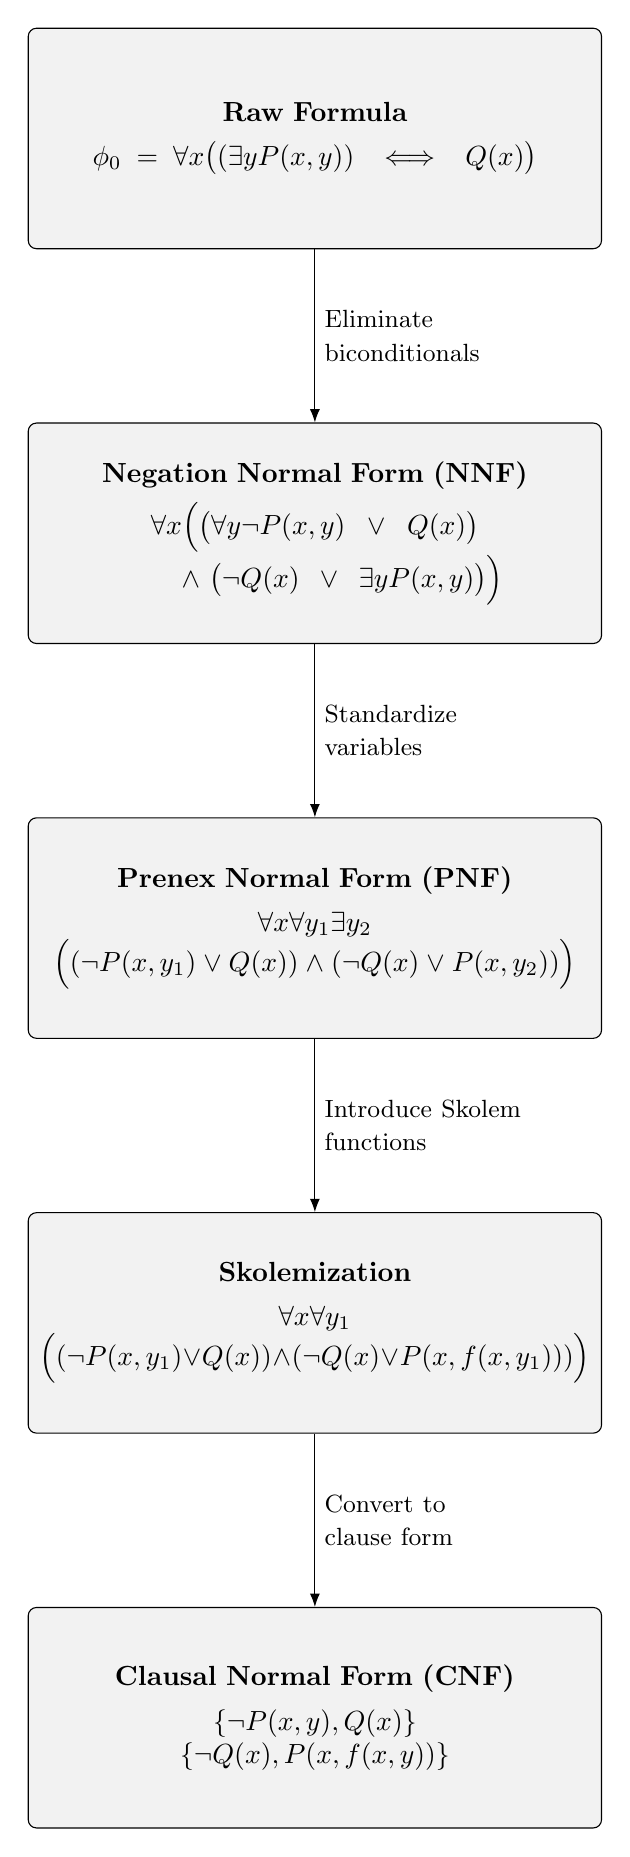
\begin{tikzpicture}[
      node distance=2.2cm and 0.8cm,
      stage/.style={draw, rounded corners=3pt, fill=gray!10, align=center, inner sep=4pt, minimum height=2.8cm},
      >=Latex
    ]

    % Nodes arranged vertically for better readability
    \node[stage, text width=7cm] (raw) {\textbf{Raw Formula} \\[4pt]
      \(\displaystyle \phi_0 = \forall x\ms\big(\ms(\exists y\ms P(x,y)) \iff Q(x)\ms\big)\)};

    \node[stage, below=of raw, text width=7cm] (nnf) {\textbf{Negation Normal Form (NNF)}\\[4pt]
      \(\displaystyle \forall x\ms\Big(\big(\forall y\ms\neg P(x,y)\ \lor\ Q(x)\big)\) \\
      \(\displaystyle \qquad\land\ \big(\neg Q(x)\ \lor\ \exists y\ms P(x,y)\big)\Big)\)};

    \node[stage, below=of nnf, text width=7cm] (pnf) {\textbf{Prenex Normal Form (PNF)}\\[4pt]
      \(\displaystyle \forall x\ms\forall y_1\ms\exists y_2\ms\)\\
      \(\displaystyle \Big((\neg P(x,y_1)\lor Q(x)) \land (\neg Q(x)\lor P(x,y_2))\Big)\)};

    \node[stage, below=of pnf, text width=7cm] (sko) {\textbf{Skolemization}\\[4pt]
      \(\displaystyle \forall x\ms\forall y_1\ms\)\\
      \(\displaystyle \Big((\neg P(x,y_1)\lor Q(x)) \land (\neg Q(x)\lor P(x,f(x,y_1)))\Big)\)};

    \node[stage, below=of sko, text width=7cm] (cnf) {\textbf{Clausal Normal Form (CNF)}\\[4pt]
      \(\{\ms\neg P(x,y),\ms Q(x)\ms\}\)\\
      \(\{\ms\neg Q(x),\ms P(x,f(x,y))\ms\}\)};

    % Arrows
    \draw[->] (raw) -- node[right, text width=3cm, align=left]{\small Eliminate\\biconditionals} (nnf);
    \draw[->] (nnf) -- node[right, text width=3cm, align=left]{\small Standardize\\variables} (pnf);
    \draw[->] (pnf) -- node[right, text width=3cm, align=left]{\small Introduce Skolem\\functions} (sko);
    \draw[->] (sko) -- node[right, text width=3cm, align=left]{\small Convert to\\clause form} (cnf);

  \end{tikzpicture}
  \caption{Pipeline: Raw formula \(\rightarrow\) NNF \(\rightarrow\) PNF \(\rightarrow\) Skolemization \(\rightarrow\) CNF.}\label{fig:nnf-to-cnf-pipeline}
\end{figure}


Transforming formulae into CNF is a prerequisite for many automated reasoning techniques, particularly \textit{resolution}~\cite{chang1997}.  
By ensuring that the input is in a uniform syntactic format, inference rules can be applied in a purely mechanical way without further structural transformations.

This pipeline of transformations, combined with \textit{naming} is what consitute the \textbf{preprocessing} phase of automated reasoning systems, a crucial step to prepare formulae for \textit{inferences}.



\section{Naming}

% \section{Typography \& maths}
% Some text here. \(\varphi,\phi,\psi\vDash M U k\)
% Here \texttt{true type}. 
% \textsc{here Small Caps}. 
% \textsf{here sans serif}. 
% \emph{here italics}.
% \textbf{\emph{here bold italics}}.
% \textbf{\textsf{bold sans}}.
% \textsf{\emph{Italic sans}}.
% %Here we cite \citeauthor{dijkstra1972humbleprogrammer} and \citeauthor{lamport1982proving}
% %who wrote \cite{dijkstra1972humbleprogrammer,lamport1982proving} respectively.
% \blindmathpaper

% \section{TODOs}
% The \texttt{uninathesis} documentclass provides a basic todo functionality via 
% the \texttt{uninatodo} command \uninatodo{as i just did. This is a todo note.}. 

% \section{Lists}
% In this section you can see how lists look like.
% \subsection{Itemize}
% \blinditemize
% \subsection{Enumerate}
% \blindenumerate
% \subsection{Description}
% \blinddescription
% \subsection{Custom enumerate}
% \begin{enumerate}[label=(\roman*)]
%     \item foo;
%     \item bar;
%     \item foobar.
% \end{enumerate}
% \subsection{Inline enumerate}
% You can also write inline enumerates as follows:
% \begin{enumerate*}[label=(\roman*)]
%     \item first item;
%     \item second item;
%     \item third and last item.
% \end{enumerate*}

% \section{Tables}
% Classic booktabs tables as in Table \ref{tab:table}. \blindtext
% \begin{table}
%     \begin{center}
%       \caption{Table using booktabs.}
%       \label{tab:table}
%       \begin{tabular}{llr}
%         \toprule % <-- Toprule here
%         \textbf{Value 1} & \textbf{Value 2} & \textbf{Value 3}\\
%         $\alpha$ & $\beta$ & $\gamma$ \\
%         \midrule % <-- Midrule here
%         1 & 1110.1 & a\\
%         2 & 10.1 & b\\
%         3 & 23.113231 & c\\
%         \bottomrule % <-- Bottomrule here
%       \end{tabular}
%     \end{center}
% \end{table}

% \section{Algorithms}
% Algorithm environment is styled to be consistent with booktabs (same heading and bottomline). \blindtext[2]
% \begin{algorithm}
%     \caption{Box alignment procedure}\label{alg:padding}
%     \begin{algorithmic}[1]
%         \Statex \textbf{signature} $\textsc{BoxAlign}$ $CSA\times CSA \to CSA\times CSA$
%         \Statex \textbf{ensure} The returned CSA are box-compatible
%         \Function{$\textsc{BoxAlign}$}{$\mathscr{M},\mathscr{F}$}
%             % I cut a whole part of the algorithm; It doesn't make much sense now!
%             \State $(\mathscr{M}^\prime,\mathscr{F}^\prime)\gets(\mathscr{M},\mathscr{F})$
%             \ForAll{$(b_m,b_f)\in B_{\mathscr{M}^\prime}\times B_{\mathscr{F}^\prime}$}
%                 \State $\left(\beta_{\mathscr{M}^\prime},\beta_{\mathscr{F}^\prime}\right)\gets(\varepsilon,\varepsilon)$
%                 \For{$0\le i < |\beta_{\mathscr{M}^\prime}(b_m)|$} 
%                     \State $(\mathscr{A}_\mathscr{M},\mathscr{A}_\mathscr{F})\gets\textsc{BoxAlign}(\beta_{\mathscr{M}^\prime}(b_m)_i,\beta_{\mathscr{F}^\prime}(b_f)_i)$
%                     \State $\beta_{\mathscr{M}^\prime}(b_m)\gets\beta_{\mathscr{M}^\prime}\cdot\mathscr{A}_\mathscr{M}$
%                     \State $\beta_{\mathscr{F}^\prime}(b_f)\gets\beta_{\mathscr{F}^\prime}\cdot\mathscr{A}_\mathscr{F}$
%                 \EndFor
%             \EndFor
%             \State \textbf{return} $(\mathscr{M}^\prime,\mathscr{F}^\prime)$
%         \EndFunction
%     \end{algorithmic}
% \end{algorithm}


% \section{Listings}
% Listings provided by the lstlistings package. Example shown in Listing \ref{lst:code}. \blindtext[2]
% \begin{lstlisting}[language=Python,float,caption=Python example,label={lst:code},basicstyle=\ttfamily,frame=b,framextopmargin=.2ex]
%     import numpy as np
     
%     def incmatrix(genl1,genl2):
%         m = len(genl1)
%         n = len(genl2)
%         M = None #to become the incidence matrix
%         VT = np.zeros((n*m,1), int)  #dummy variable
     
%         #compute the bitwise xor matrix
%         M1 = bitxormatrix(genl1)
%         M2 = np.triu(bitxormatrix(genl2),1) 
% \end{lstlisting}


% \section{Listings, Algorithm and Table: consistent styling}
% The section title and Figure \ref{fig:figure} are pretty self-explanatory.\Blindtext
% \begin{figure}\centering
% \begin{minipage}[t]{.3\textwidth}
% \begin{algorithm}[H]
%     \caption{Test}
%     \begin{algorithmic}[1]
%         \State $z\gets 1+1$
%         \State $z\gets 1+2$
%     \end{algorithmic}
% \end{algorithm}
% \end{minipage}\hfill
% \begin{minipage}[t]{.3\textwidth}%
%     \vspace{.7em}
%     \begin{lstlisting}[language=Python,caption=ex]
%     int foo;
%     foo=1;
%     \end{lstlisting}
% \end{minipage}\hfill%
% \begin{minipage}[t]{.3\textwidth}
% \begin{table}[H]
%     \begin{tabular}{ll}
%         \toprule
%         foo & bar \\
%         \midrule 
%         1 & 2 \\
%         \bottomrule
%     \end{tabular}
% \end{table}
% \end{minipage}
% \caption{Algorithm, code and table side by side}\label{fig:figure}
% \end{figure}

    %\chapter{Second chapter}

\blindmathpaper

   % other chapters here..

    % \newpage\pagestyle{conclusions}
\chapter*{Conclusions}

\blindtext

\unnumberedsection{Some section}
\blindtext

\unnumberedsection{Some other section}
\blindtext

    % %appendix title style
\titleformat{\chapter}[block]{\Huge\bfseries}{
    \sffamily\huge\centering{Appendix \thechapter
}\\}{1ex}{\sffamily\centering\huge\bfseries}

\newpage\pagestyle{appendices}
\begin{appendices}

\chapter{This is an appendix}\label{appendix}
\section{Appendix section}
\Blindtext
\section{Appendix section}
\Blindtext

%now another appendix
\blinddocument
\end{appendices}
    
    \newpage
    \pagestyle{backmatter}
    \printbibliography[heading=bibintoc]
    

    %\listoffigures
 
    %\listoftables

\end{document}